\documentclass[a4paper,12pt]{article}
\usepackage{graphicx,textcomp,amsmath,amssymb,IEEEtrantools,adjustbox,wrapfig,chngcntr,tikz,float,amsthm,listings,caption,enumitem,caption,subcaption,siunitx,booktabs,multirow,array,cancel}
\usepackage[toc,page]{appendix}

%BACKLINK SETUP FOR CLICKABLE LINKS
\usepackage{hyperref}
\hypersetup{
    colorlinks,
    citecolor=blue,
    filecolor=blue,
    linkcolor=blue,
    urlcolor=blue
}
%END-BACKLINK SETUP FOR CLICKABLE LINKS

\usepackage{pgfplots}

\pgfplotstableread{
x         y    y-max  y-min
0.5  20.52 0.91   0.91
0.6 24.01 0.78   0.78
0.7     27.56 1.05   1.05
0.8 31.92 0.79 0.79
0.9 36.00 1.32 1.32
1.0 39.94 1.52 1.52
}{\mytable}

\pgfplotstableread{
x         y    y-max  y-min
0.5  0.83 0.04 0.04
0.6 0.96 0.04 0.04
0.7 1.10 0.04 0.04
0.8 1.28 0.02 0.02
0.9 1.44 0.05 0.05
1.0 1.59 0.05 0.05
}{\myothertable}


\usepackage{parskip}
\usepackage{indentfirst}

\usepackage{fancybox} 


\definecolor{codegreen}{rgb}{0,0.6,0}
\definecolor{codegray}{rgb}{0.5,0.5,0.5}
\definecolor{codepurple}{rgb}{0.58,0,0.82}
\definecolor{backcolour}{rgb}{0.95,0.95,0.92}

%WHEN DOES EQUATION COUNTER CHANGE
\counterwithin{equation}{section}
%END-WHEN DOES EQUATION COUNTER CHANGE

%DOUBLE SPACING IF NEEDED
%\usepackage{setspace}
%\doublespacing
%END-DOUBLE SPACING IF NEEDED


%BORDER
\usepackage[paperwidth=7.27in,paperheight=10.69in,left=0.5in, right=0.5in, top=1in, bottom=1in]{geometry}
\usepackage[a4,frame,center,noinfo]{crop}
%END-BORDER

\usepackage{fancyhdr}
\pagestyle{fancy}
\fancyhead{}
\renewcommand{\headrulewidth}{0pt}
\usepackage{blindtext}
\usepackage{lastpage}
\rfoot{Page{} \thepage\ of \pageref{LastPage}}
\cfoot{}
\chead{\footnotesize{To what extent does length of string %and distance of suspension 
effect the time period and subsequently the rotational inertia of a bifilar pendulum?}}



%PARAGRAPH INDENTATION
\setlength{\parskip}{1em}
\setlength{\parindent}{1cm}
%END-PARAGRAPH INDENTATION

\binoppenalty=10000
\relpenalty=10000

\newtheorem{theorem}{Theorem}
\theoremstyle{definition}
\newtheorem{definition}{Definition}

\begin{document}

%TITLE PAGE
\begin{titlepage}
    \begin{center}
    
        \vspace*{0.2cm}
 
        \Large
        \textbf{Physics Exploration}
        
 		\textbf{Higher Level}

        

        \vspace{2.5cm}
		
		
		\textbf{Exploration Title: }To what extent does length of string %and distance of suspension
		 affect time period  and subsequently the rotational inertia of a bifilar pendulum?
 
        \vfill
 
 
        \vspace{0.8cm}

 
    \end{center}
\end{titlepage}
%END-TITLE PAGE





\section{Introduction}
Pendulums are instruments crucial to many of our day-to-day activities. Everything from clocks to accelerometers use pendulums. A pendulum can be broadly defined as a weight suspended from a fixed point or pivot allowing for it to swing freely.

As a child, and even today, one of my favorite things to do at a playground is to swing. Soon I realized the swing could be viewed as one version of the pendulum. It is the bifilar or doubly suspended pendulum. Commonly known as a ``swing" to children all around the world, this type of pendulum consists of two parallel strings of equal length known as filars which suspend a longitudinal mass. 

\begin{figure}[h]
\centering
\begin{subfigure}{.5\textwidth}
  \centering
  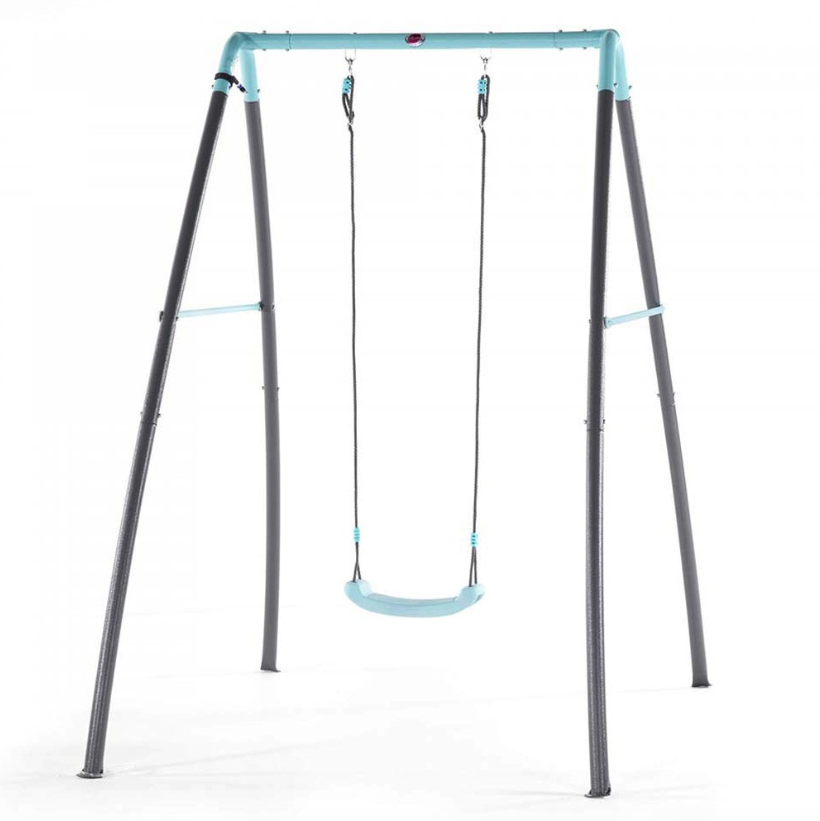
\includegraphics[width=.8\linewidth,height=10cm,keepaspectratio]{swing}
  \caption{}
  \label{fig:sub1}
\end{subfigure}%
\begin{subfigure}{.5\textwidth}
  \centering
  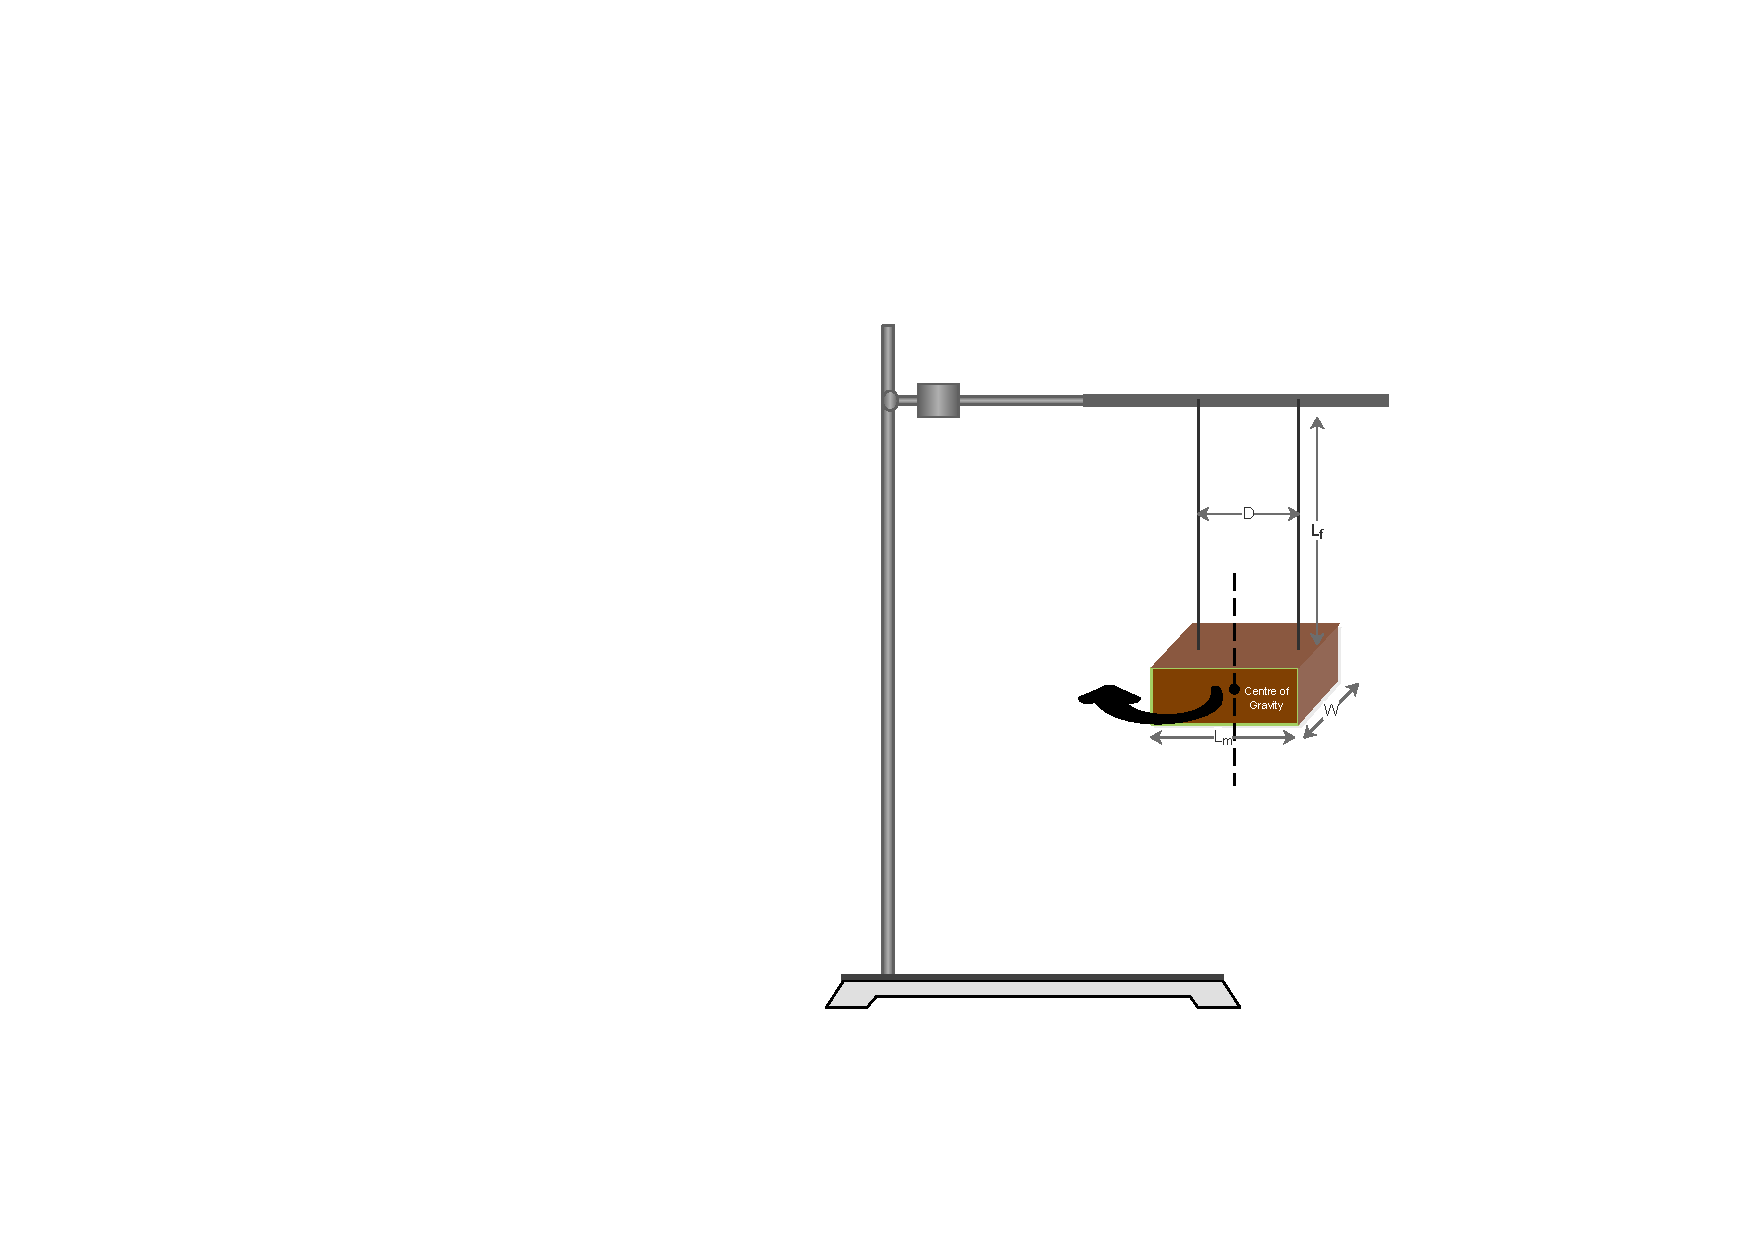
\includegraphics[width=.7\linewidth,height=10cm,keepaspectratio]{setup.pdf}
  \caption{}
  \label{fig:sub2}
\end{subfigure}
\caption{Children's swing and bifilar pendulum}
\label{fig:test}
\end{figure}




If a bifilar pendulum is suspended by a rigid point at both filars, and is made to oscillate in direction perpendicular to its suspension, to create moment, there is a rotation inertia ($I$) that can be calculated experimentally using\footnote{Mitiguy, Paul, et al. ``Rotational Systems." \textit{ME161: Dynamic Systems,} Stanford University, 2017, web.stanford.edu/class/me161/labs/Lab03RotationalSystems.pdf. Accessed on: 19 Feb. 2019.},
\begin{equation}\label{eq:experimental}
	I=\frac{mgT^2 D^2}{(4\pi)^2 L_f}
\end{equation}
(where $m$ is the mass of the suspended object, $g$ is the constant of acceleration due to gravity, $T$ is the time period of 1 oscillation, $D$ is the length between where the string attaches and the centre of gravity, and $L_f$ is the length of the filar)

Although, inertia is a property of all matter. It is the resistance to a change in motion and is inherently a property of mass. Therefore, a moment of inertia is created when a force is applied at a distance to the point of rotation, resulting in torque. Moment of Inertia (MoI) is also known as Rotational Inertia. Therefore, the moment of inertia can be calculated for any object that has a mass. For example, the theoretical MoI for a cuboid is\footnote{Serway, ``Raymond A. Physics for Scientists and Engineers." \textit{Saunders College Pub.}, 1986.},
\begin{equation}\label{eq:theorectical}
	I = \frac{1}{12}m(W^2+L_m^2)
\end{equation}
(where $m$ is the mass of the cuboid, $W$ is the width, and $L_m$ is the length)

\begin{figure}[h]
    \centering
    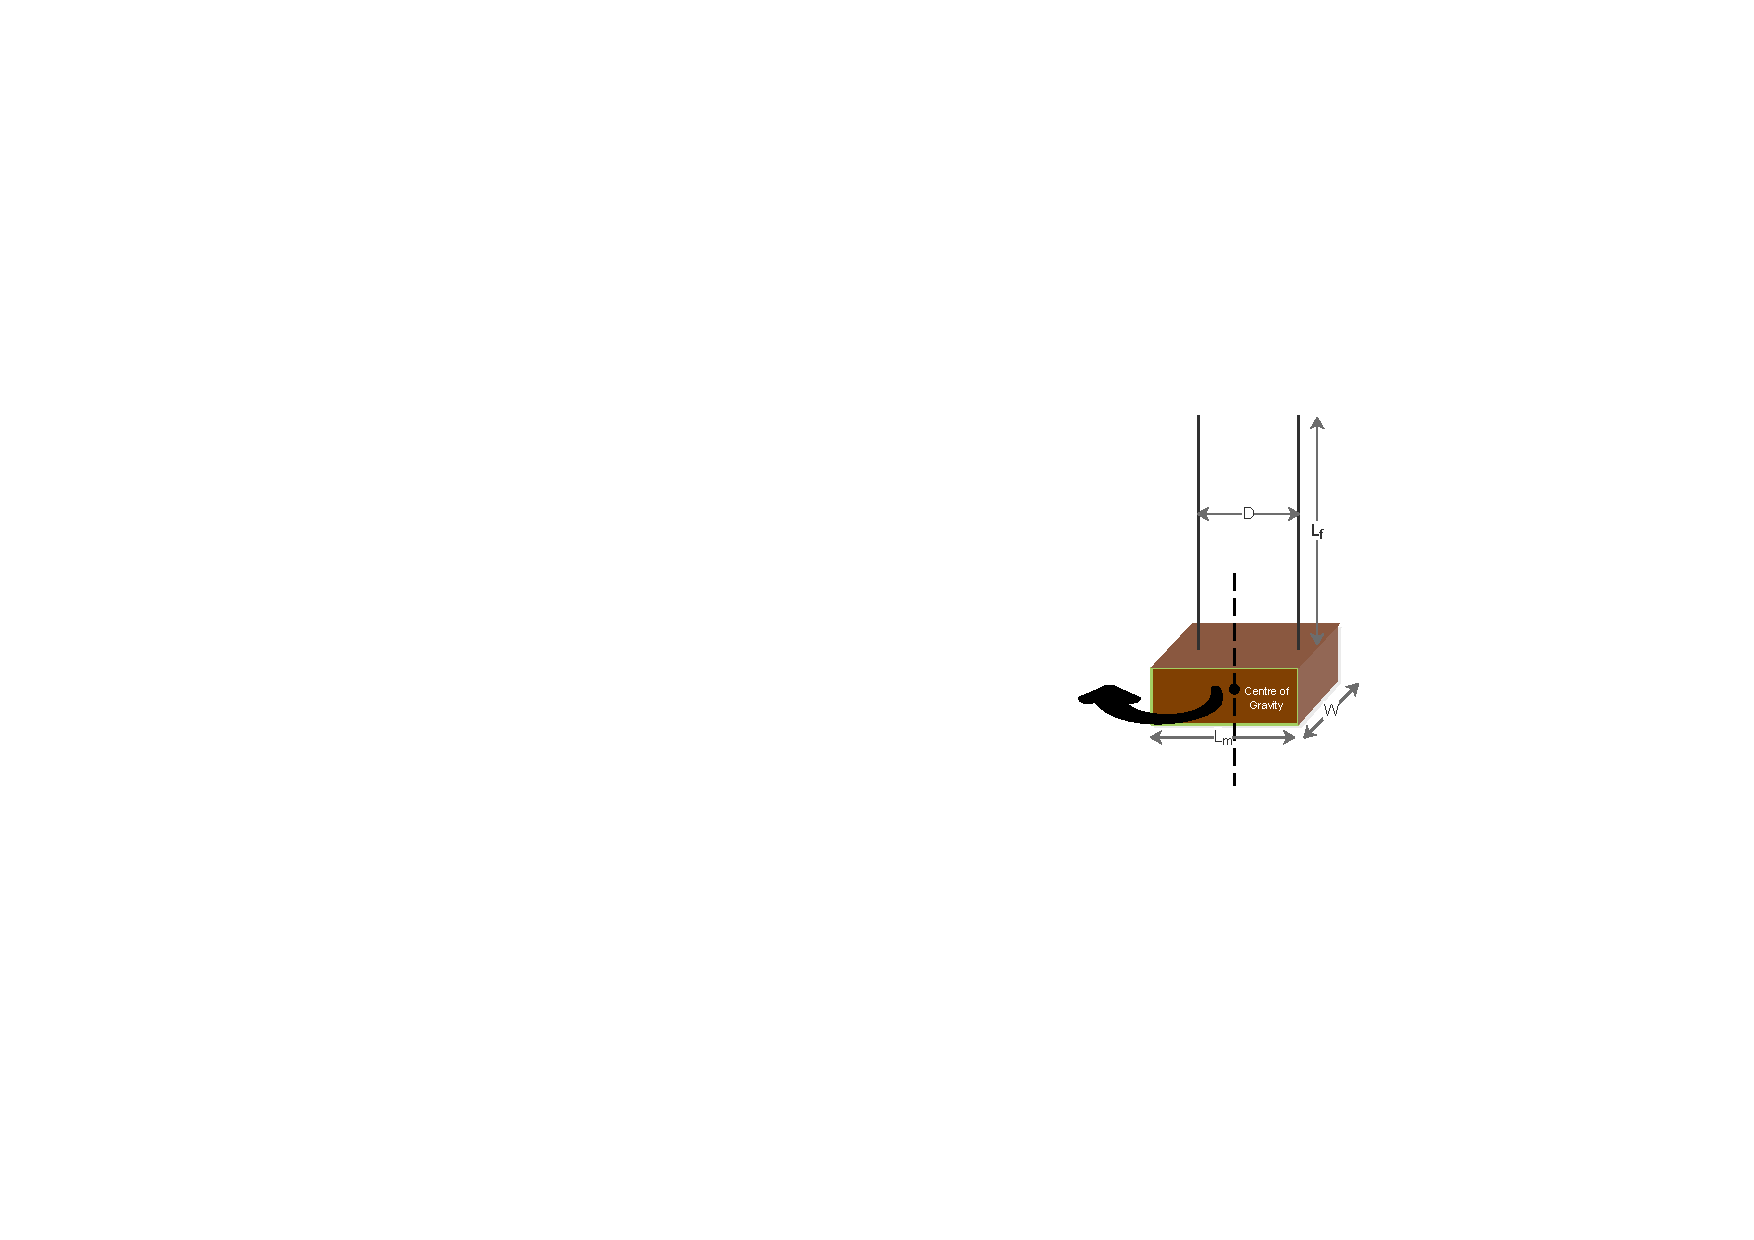
\includegraphics[width=\textwidth,height=10cm,keepaspectratio]{setup2.pdf}
    \caption{Dimensions of experimental setup}
    \label{fig:measurements}
\end{figure}

It is also interesting to note the other applications of bifilar pendulums. Currently they are being used to study the mass moment of inertia on aircrafts and UAVs (unmanned air vehicles)\footnote{Jardin, Matthew, and Eric Mueller. ``Optimized measurements of UAV mass moment of inertia with a bifilar pendulum." \textit{AIAA Guidance, Navigation and Control Conference and Exhibit,} 2007.}. Furthermore, the idea of a bifilar pendulum can be applied to studying suspension bridges and how they react to disturbances due to wind, load, angle of spacing between filars, and length of filar\footnote{Nester, Tyler M., et al. ``Experimental observations of centrifugal pendulum vibration absorbers." \textit{International Symposium on Transport Phenomena and Dynamics of Rotating Machinery,} 2004.}. In order to investigate this, my experiment varies the length of the filars and the distance of suspension of filars to see how it effects the time period of a bifilar pendulum\footnote{Then, John W., and Kang-rong Chiang. ``Experimental determination of moments of inertia by the bifilar pendulum method." \textit{American Journal of Physics,} 1970.}.

\newpage
\section{Design}
\parskip0.5em

	\subsection{Research Question}

	To what extent does length of string effect the time period and subsequently the rotational inertia of a bifilar pendulum?
	
	\subsection{Hypothesis}
	
	
	The period $T$ will become longer and the length of the filars $L_f$ is increased. There will be a linear relationship between $T^2$ and $L$ based on equation \ref{eq:experimental}. Rotational inertial can be empirically measured using the time period and length of string, and will get more accurate as length of string increases\footnote{Jardin, Matt R., and Eric R. Mueller. ``Optimized measurements of unmanned-air-vehicle mass moment of inertia with a bifilar pendulum." \textit{Journal of Aircraft,} 2009.}.

	
	\subsection{Parameters}
	
	\begin{enumerate}
		\item Independent Variable: length of filar ($L_f$) in meters (\si{m})
			%\item distance between filars ($D$) in meters ($m$)
		
		\item Dependent Variable: rotational time period $T$ in seconds (\si{s})
		
		\item Controlled Varibales:
	
	
\begin{table}[!h]
\begin{tabular}{|p{=3cm}|p{6cm}|p{6cm}|}
\hline
\textbf{Variable}             & \textbf{Reason}                                                                                                          & \textbf{Method} \\ \hline
Mass and dimensions of object & Objects with different masses and dimensions would have different period of oscillation, and therefore different inertia & Only one rectangular object was used for the whole experiment and rotated in the same degree                \\ \hline
String                        & Strings in different materials, or different thickness (radius) could affect the inertia and time period                 & String of same thickness and material was used. The length was varied as the IV               \\ \hline
Angle of string               & If the strings are not parallel, the oscillations could be disturbed and unusual                                                                                                                         & Strings of the same length are used and connected equidistant to the centre of of mass of the object                \\ \hline
Wind                          & External forces such as wind could disrupt the regular oscillations with swaying motions                                                                                                                          & Windows and doors in the laboratory were shut during the experiment                \\ \hline
Distance between strings      &    Varied distances between strings would change the effect on the centre of mass, and therefore the rotation                                                                                                                      &   Holes were drilled into the wooden rectangular object so that distance between strings was constant              \\ \hline
\end{tabular}
\end{table}
\end{enumerate}


\subsection{Procedure}


\begin{enumerate}
	\item Holes were drilled into a rectangular wooden block (weghing \SI{1}{kg}, \SI{0.500}{m} long, wide \SI{0.040}{m}) equidistant from the sides and the center. 
	\item Strings were passed into each of the holes, and firmly tied so they would not pass through the hole in the block.
	\item Strings were attached parallel to the hook clamps on the support.
	\item Using a protractor, the block was let spun to \ang{180}, and then let go.
	\item At the exact moment the disk was released, the stopwatch was started. The stopwatch reading was taken after 5 periods, 5 times in one spin.
	\item Steps 4 to 5 were repeated 3 times. 
	\item Steps 2 to 6 were repeated for lengths of strings \SIlist{0.500;0.600;0.700;0.0800}{\meter}.
\end{enumerate}


\subsection{Apparatus}
\begin{figure}[h]
    \centering
    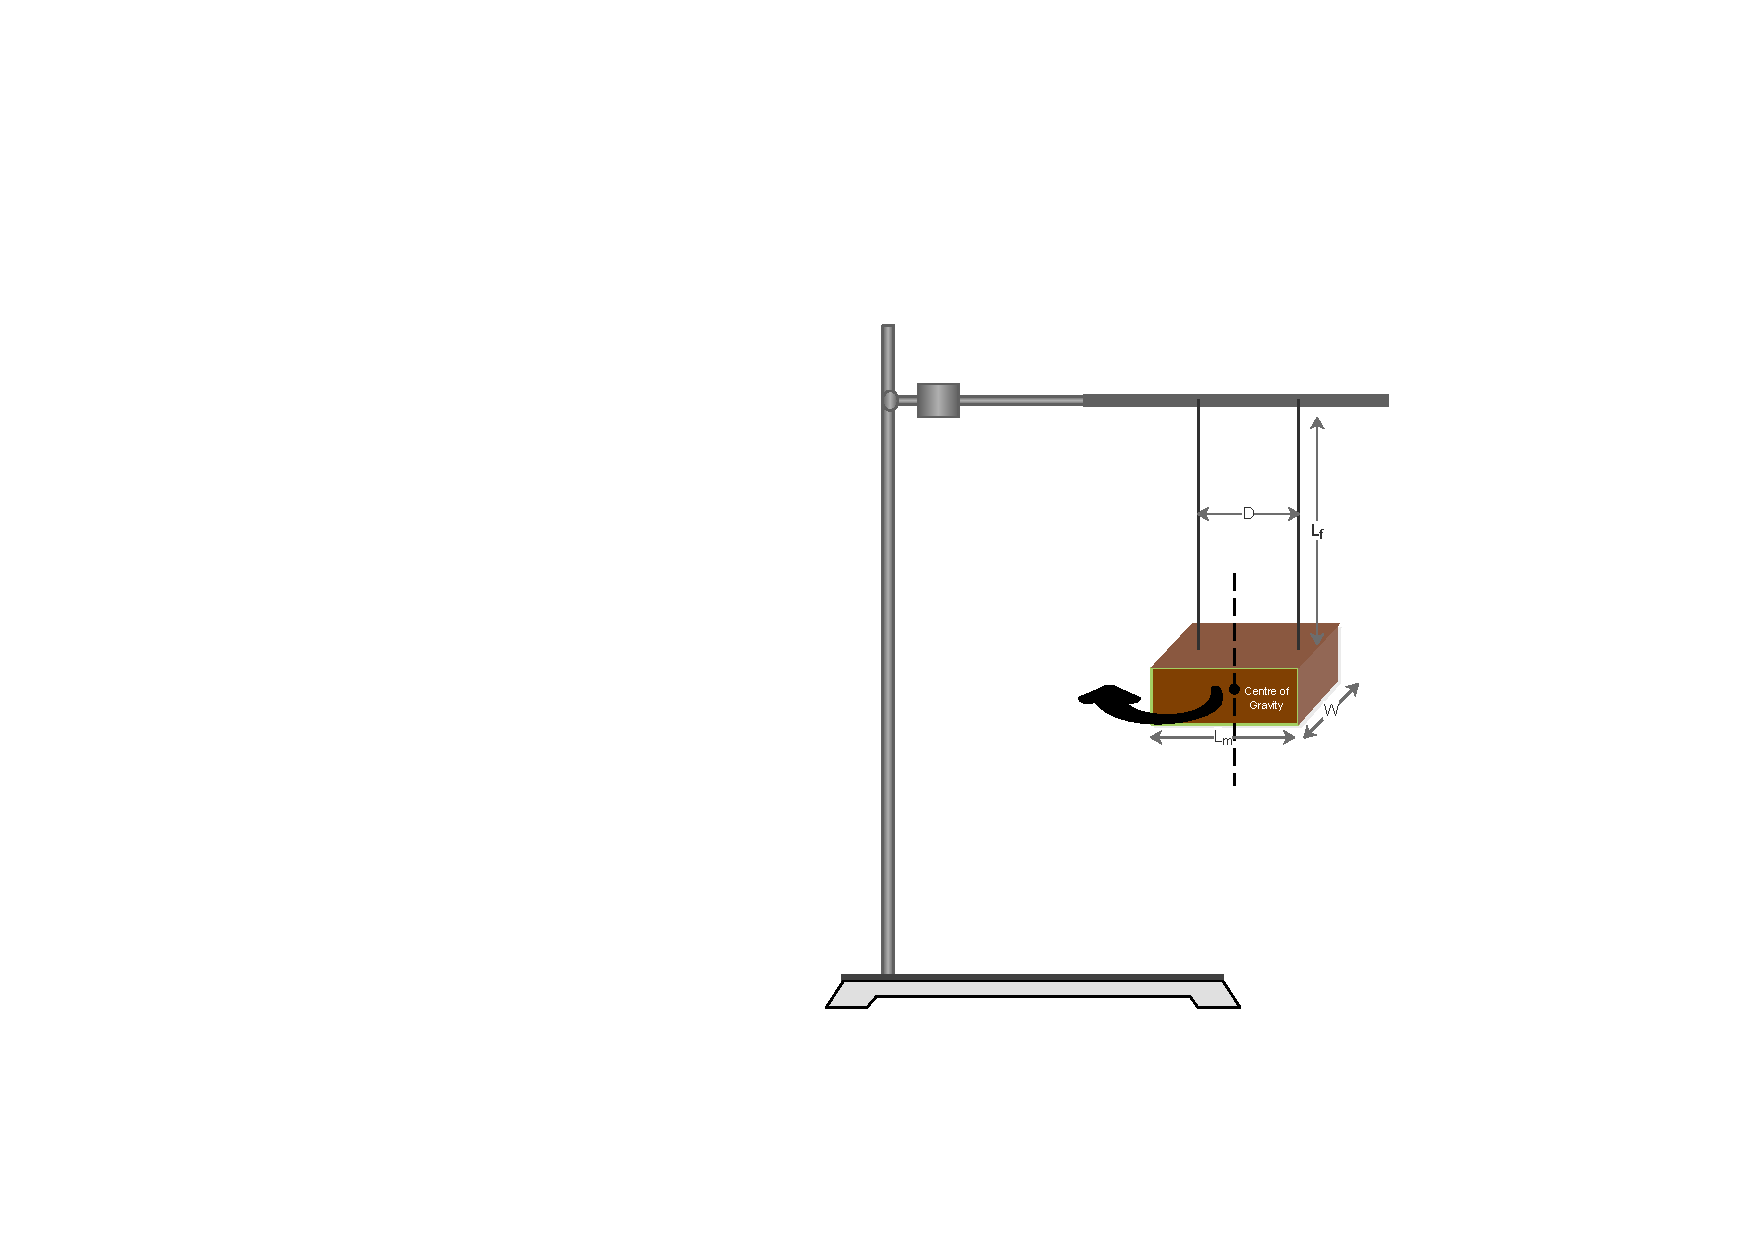
\includegraphics[width=\textwidth,height=10cm,keepaspectratio]{setup.pdf}
    \caption{Apparatus}
    \label{fig:apparatus}
\end{figure}



\newpage
\section{Data collection and analysis}
\subsection{Raw data}


\setlength{\extrarowheight}{5pt}
\begin{table}[h]
\begin{center}
\begin{tabular}{l||c|llllll} \toprule
\multicolumn{2}{l||}{$L(\si{\m}) \pm 0.0005 \si{\m}$ }      & 0.500 & 0.600 & 0.700 & 0.800 & 0.900 & 1.000 \\ \midrule
\parbox[t]{2mm}{\multirow{15}{*}{\rotatebox[origin=c]{90}{$t(\si{\s}) \pm 0.01 \si{s}$}}} 
								   & $t_1$ &   4.57    &  4.83     &   5.21    &   5.59 & 6.03  &6.36\\
                                   & $t_2$ &    4.49   &  4.98     &     5.16  &    5.62 & 6.06 &6.40\\
                                   & $t_3$ &   4.56    &   4.87    &     5.36  &     5.65 & 6.13&6.24\\
                                   & $t_4$ &   4.49    &   4.89    &     5.26  &    5.61 &  5.94&6.32\\
                                   & $t_5$ &   4.51    &    4.88   &     5.28  &   5.70  & 5.99 &6.33\\ 
                                   & $t_6$ &   4.50    &   4.97    &   5.21    &  5.69  &  5.92 &6.19\\
                                   & $t_7$ &     4.51  &    4.90   &    5.20   &   5.64  &  5.94&6.38\\
                                   & $t_8$ &     4.59  &    4.89   &   5.16    &    5.68 &  6.03&6.37\\
                                   & $t_9$ &     4.60  &    4.86   &    5.28   &   5.62  & 6.06 &6.36\\
                                   & $t_{10}$ &    4.51   &    4.86   &    5.26   & 5.66 &   5.94& 6.41 \\ 
                                   & $t_{11}$ &   4.46    &    4.91   &  5.24     &  5.61 & 5.95  & 6.27\\
                                   & $t_{12}$ &   4.65    &    4.91   &   5.22    &  5.69  &  6.07 &6.18\\
                                   & $t_{13}$ &    4.53   &   4.94    &   5.33    &  5.70  &  6.05 &6.21\\
                                   & $t_{14}$ &   4.44    &    4.98   &    5.30   &  5.61  &  5.93 &6.41\\
                                   & $t_{15}$ &     4.50  &     4.88  &   5.26    &   5.73 &  5.94&6.35\\ \bottomrule
\end{tabular}
\end{center}
\caption{Raw data with time ($t$) for 5 oscillations}
\label{tab:rawdata}
\end{table}

\subsection{Processed data}
With the data presented in Table \ref{tab:rawdata}, it is important to calculate the mean time for 5 oscillations ($t_{avg}$) for each sets of readings for each length of filar (string). It must be noticed that the values presented in Table \ref{tab:rawdata} are the time periods for 5 oscillations, therefore the time period for 1 oscillation will be,
\begin{equation}
	T_{osc}=\frac{t_n}{5}
\end{equation} 
(where $t_n$ is any time period in Table \ref{tab:rawdata})

To calculate the mean, the following formula is used,
\begin{equation}
	t_{avg} = \frac{\sum\limits_{n=1}^{15} t_n}{N}=\frac{t_1+t_2+t_3 + ... + t_{13} + t_{14} + t_{15}}{15}
\end{equation}

When calculating mean, an uncertainty is present. This can be calculated as,
\begin{equation}
	\Delta t_{avg}=\frac{Range}{2}=\frac{t_{max}-t_{min}}{2}
\end{equation} 

For example, for $L=\SI{0.500}{m}$, 
\begin{equation}
	t_{avg} = \frac{\sum\limits_{n=1}^{15} t_n}{N}=\frac{67.91}{15}=4.527333 \approx \SI{4.53}{s}
\end{equation}
\begin{equation}
	\Delta t_{avg} = \frac{4.64-4.44}{2}\approx \SI{0.10}{s}
\end{equation}

\setlength{\extrarowheight}{3pt}
\begin{table}[h]
\begin{center}
\begin{tabular}{l||c|ll|ll} \toprule
\multicolumn{2}{l||}{Time period (\si{s}) }   &  $t_{avg}$ & $\Delta t_{avg}$ & $T_{osc}$ & $\Delta T_{osc}$ \\ \midrule
\parbox[t]{2mm}{\multirow{5}{*}{\rotatebox[origin=c]{90}{$L(\si{\m}) \pm 0.0005 \si{\m}$}}} 
								   & \SI{0.500}{m}     &  4.53 & $\pm$ 0.10 &  0.91 &  $\pm$ 0.02\\
                                   & \SI{0.600}{m}    &  4.90 & $\pm$ 0.08 & 0.98 & $\pm$ 0.02\\
                                   & \SI{0.700}{m}    &    5.25 & $\pm$ 0.10  & 1.05 & $\pm$ 0.02\\
                                   & \SI{0.800}{m}     &   5.65 & $\pm$ 0.07   &  1.13 & $\pm$ 0.01\\
                                   	& \SI{0.900}{m}     &   6.00 &$\pm$ 0.11   & 1.20 & $\pm$ 0.02\\
                                   	& \SI{1.000}{m}     &   6.32 &$\pm$ 0.12   & 1.26 & $\pm$ 0.02\\
                       
\bottomrule
\end{tabular}
\end{center}
\caption{Average of $t_n$ and  singular oscillation period ($T_{osc}$)}
\label{tab:processeddata}
\end{table}

Rearranging equation \ref{eq:experimental} to make $T^2$ the subject, the relationship between time period ($T_{osc}$) and length of the string or filar becomes noticeable.
\begin{equation}\label{eq:timeassubject}
	T^2=\frac{(4 \pi)^2 \cdot I \cdot L}{m \cdot g \cdot D^2}
\end{equation}

For example, the calculation of $(t_{avg} \pm \Delta t)^2$ for \SI{0.800}{m} requires the calculation of $t_{avg}^2$ first as follows:
\begin{equation*}
	t_{avg}^2 = (\SI{5.65}{s})^2=\SI{31.9225}{s^2} \approx \SI{31.93}{s}
\end{equation*}

Which prompts the calculation of $\Delta t_{avg}^{2}$ as,
\begin{equation}
	\Delta t_{avg}^{2}=\frac{2 \cdot \left( \frac{\Delta t_{avg}}{t_{avg}}\times \cancel{100} \right) }{\cancel{100}}\times t_{avg}^2 ={2 \cdot \left( \frac{\Delta t_{avg}}{\cancel{t_{avg}}} \right) } \times t^{\cancel{2}}_{avg} = 2\cdot \Delta t_{avg}\cdot t_{avg}
\end{equation}\label{eq:squareuncertainty}
For example, the $\Delta t_{avg}^2$ for \SI{0.800}{m} is,
\begin{equation*}
	\Delta t^2_{avg} = 2 \cdot 0.07 \cdot 5.65  \approx \SI{0.79}{s^2}
\end{equation*}
Similarly or all $t^2_{avg}$ and $T^2_{osc}$ for all measured lengths $L$ with uncertainty calculated through equation \ref{eq:squareuncertainty},
\begin{table}[H]
\begin{center}
\begin{tabular}{l||c|ll|ll} \toprule
\multicolumn{2}{l||}{Time (\si{s^2}) }   &  $t_{avg}^2$ & $\Delta t_{avg}^2$  & $T_{osc}^2$ & $\Delta T_{osc}^2$\\ \midrule
\parbox[t]{2mm}{\multirow{5}{*}{\rotatebox[origin=c]{90}{$L(\si{\m}) \pm 0.0005 \si{\m}$}}} 
								   & \SI{0.500}{m}     &  20.52 & $\pm$ 0.91 & 0.83&$\pm$ 0.04\\
                                   & \SI{0.600}{m}    &  24.01 &$\pm$ 0.78 & 0.96&$\pm$ 0.04\\
                                   & \SI{0.700}{m}    &    27.56 &$\pm$ 1.05 & 1.10&$\pm$ 0.04 \\
                                   & \SI{0.800}{m}     &   31.92 &$\pm$ 0.79 &1.28 &$\pm$ 0.02\\
                                   	& \SI{0.900}{m}     &   36.00 &$\pm$  1.32 &1.44 &$\pm$ 0.05\\
                                   		& \SI{1.000}{m}     &   39.94 &$\pm$  1.52 &1.59 &$\pm$ 0.05\\
                       
\bottomrule
\end{tabular}
\end{center}
\caption{Relationship between $L$ and $t^2_{avg}$ or $T^2_{osc}$}
\label{tab:processeddatasquare}
\end{table}

If equation \ref{eq:timeassubject} is plotted for squared time period, $T^2$, against length of filar, $L$, it should give a linear graph correlating $T^2$ and $L$ with gradient as $\frac{(4 \pi)^2 I}{mgD^2}$.


\begin{figure}[H]
\centering
\begin{tikzpicture}[scale=1.05, transform shape]
\begin{axis} [
	xlabel={Length of filar (m)},
    ylabel={Time period squared ($s^2$)},
    ymin=0,
    xtick=data,
    minor tick num=5,
    grid=both,
    grid style={line width=0.5pt, draw=gray!10},
    major grid style={line width=.2pt,draw=gray!50},
    legend pos=north west,
]
\addplot [only marks] 
  plot [error bars/.cd, y dir=both, y explicit]
  table [y error plus=y-max, y error minus=y-min] {\myothertable};
\addplot[
    color=blue,
    ]
    coordinates {
    (0.5,0.83)(0.6,0.961)(0.7,1.10)(0.8,1.28)(0.9,1.44)(1.0,1.59)
    };
    \legend{$T_{osc}^2$};
\end{axis} 
\end{tikzpicture}
\caption{Time period squared ($T_{osc}^2$) against length of filar ($L$)}
\label{fig:correlation2}
\end{figure}

As discussed, the gradient ($k$) of figure \ref{fig:correlation2} which plots time period of 1 oscillation $T_{osc}$ should give us the value of $\frac{(4 \pi)^2 I}{mgD^2}$, which is constant for this mass. It can be empirically found as, 
\begin{equation}\label{eq:empiricalgradient}
	k = \frac{1.59-0.83 \text{ s}^2}{1.0-0.5 \text{ m}} = \frac{0.76 \text{ s}^2}{0.5 \text{ m}} \approx \SI{1.52}{\second^2\per\metre} 
\end{equation}
This can be compared to the theoretical value of $\frac{(4 \pi)^2 I}{mgD^2}$ using the theoretical inertia found using equation \ref{eq:moi} of $I \approx 0.02$ for the block of wood used in this experiment,
\begin{equation}\label{eq:theoreticalgradient}
	\frac{(4 \pi)^2 I}{mgD^2} = \frac{16 \cdot 9.97 \cdot \SI{0.02}{\kilogram.\metre^2}}{\SI{1}{kg} \cdot \SI{9.81}{m/s^2} \cdot \SI{0.21}{m^2}} \approx \SI{1.55}{s^2/m}
\end{equation}
Equations \ref{eq:empiricalgradient} and \ref{eq:theoreticalgradient} show the clear similarity between the empirical value or the gradient and the theoretical value.


\section{Evaluation}
\subsection{Coefficient of Correlation}
The correlation coefficient ($r$) of $T^{2}_{osc}$ and $L$ can be calculated from table \ref{tab:processeddatasquare} using the following formula,
\begin{equation}
	r=\frac{\sum\limits_{n=1}^{5}(L_n-\overline{L})(T^2_n-\overline{T^2})}{\sqrt{\sum\limits_{n=1}^{5}(L_n-\overline{L})}\sqrt{\sum\limits_{n=1}^{5}(T^2_n-\overline{T^2})}} \approx 0.99
\end{equation}
This high degree of correlation reiterates what we saw in figure  \ref{fig:correlation2}. There is a linear correlation between $T^2$ and $L$ as predicted by the hypothesis.



\subsection{Moment of Inertia}
As previously discussed, inertia is an inherent property of all matter. This experiment can help estimate the theoretical inertia used in the previous section and found using equation \ref{eq:theorectical},
\begin{equation}\label{eq:moi}
	I_{theo}=\frac{1}{12}\cdot \SI{1}{kg}\cdot[(\SI{0.04}{m})^2+(\SI{0.5}{m})^2]=0.0209\approx \SI{0.02}{kg.m^2}
\end{equation}
Using the singular oscillation time period, $T_{osc}$ given in Table \ref{tab:processeddata} for each of the lengths, the experimental MoI can be found using equation \ref{eq:experimental}. This can be compared to the theoretical MoI. For example, the experimental MoI for $L=\SI{0.800}{m}$ is,
\begin{equation}
	I_{emp}=\frac{\SI{1}{kg}\cdot \SI{9.81}{m/s^2} \cdot\SI{1.28}{s^2}\cdot \SI{0.21}{m^2}}{16 \cdot 9.87 \cdot \SI{0.800}{m}} = 0.02087 \approx \SI{0.02}{kg.m^2}
\end{equation}
Furthermore, MoI can also be calculated using the gradient in figure \ref{fig:correlation2} which is $k=\frac{(4 \pi)^2 I}{mgD^2}$, making the MoI $I_{grad}=\frac{kmgD^2}{(4 \pi)^2}$. For example for $L=$\SI{0.800}{m},
\begin{equation}
	I_{grad} = \frac{kmgD^2}{(4 \pi)^2} = \frac{\SI{1.52}{s^2/m} \cdot \SI{1}{kg} \cdot \SI{9.81}{m/s^2} \cdot \SI{0.21}{m^2}}{16 \cdot 9.97} = 0.019629 \approx \SI{0.02}{kg.m^2}
\end{equation}
Calculating MoI using various methods helps answer the research question of this experiment. It shows how length of filar can be changed to help more accurately calculate 

\begin{table}[H]
\begin{center}
\begin{tabular}{l||c|l|ll} \toprule
\multicolumn{2}{l||}{MoI \si{kg.m^2}}   & $I_{theo}$  & $I_{grad}$  & $I_{emp}$\\ \midrule
\parbox[t]{2mm}{\multirow{5}{*}{\rotatebox[origin=c]{90}{$L(\si{\m}) \pm 0.0005 \si{\m}$}}} 
								   & \SI{0.500}{m}     &  0.02 &  0.02 & 0.02\\
                                   & \SI{0.600}{m}    &  0.02 & 0.02 & 0.02\\
                                   & \SI{0.700}{m}    &    0.02 & 0.02  & 0.02\\
                                   & \SI{0.800}{m}     &   0.02 & 0.02 & 0.02\\
                                   	& \SI{0.900}{m}     &   0.02 &  0.02 & 0.02\\
                                   		& \SI{1.000}{m}     &   0.02 &  0.02 & 0.02\\
                       
\bottomrule
\end{tabular}
\end{center}
\caption{Theoretical vs. real values for MoI}
\label{tab:comparisionofintertialvalues}
\end{table}
Due to the low precision of the devices used to make the measurements, as well as the low time period that arose due to the use of a shorter string, the real values of the MoI could not be calculated to more precision. Regardless, even at this state they show a successful calculation of MoI precise up to 2 d.p.



\subsection{Systemic errors affecting accuracy}
\begin{table}[H]
\begin{tabular}{|p{3.4cm}|p{6.5cm}|p{5.5cm}|}
\hline
\textbf{Error}             & \textbf{Effects}                                                                                                          & \textbf{Improvements} \\ \hline
     Wind and air resistance                   &     There might have been a breeze or some resistance by the wooden block to it. Regardless, this was majorly accounted for.            &   Could be eliminated in a vacuum chamber but unnecessary for such an experiment   \\ \hline
         Uneven mass distribution of the block      & The wooden block might have had a heavier side, shifting the period calculations slightly. & Use material such as metal to get more even distribution of mass.          \\ \hline
                Friction between string and pivot and angle between strings         &    As there was nothing used to keep the filars parallel, there could have been a damping affect due to a change in angle after oscillations.                                                                                                  &   Smooth, yet sturdy pivots, that keep the filars parallel to each other at all times.           \\ \hline
   String was  made of a series of twisted fibers  &   The opposing force between fibers could have had a damping effect on the oscillations, making the time period shorter.                                                                                                                     &  Use a straight thin wire of a material not composed of loose fibers such as guitar string or copper wire. \\ \hline
\end{tabular}
\end{table}

\subsection{Random errors affecting precision}
\begin{table}[!h]
\begin{tabular}{|p{3cm}|p{6cm}|p{5cm}|}
\hline
\textbf{Error}             & \textbf{Effects}                                                                                                          & \textbf{Improvements} \\ \hline
              Human error when measuing period using stopwatch          &        This can greatly effect the results specially due to the fast period of this pendulum. There are clearly some period measurements with 0.5s different for a particular length, shown by the figure \ref{fig:correlation2} not being a completely straight line.         &   Use a light-gate or high frame-rate camera to measure the period. Or, use a longer string $L$ and longer $D$ to increase the time period of the pendulum, making the error less significant.   \\ \hline
     Angle of release          & Since only a protractor was used to measure the angle at which the wooden block was released from rest, there might be great differences in each trial conducted. Regardless, this would not greatly affect period at all.&   A smartphone equipped with a compass or a regular compass could be used to release the mass at the exact specific angle every time, even though it does not make a significant difference.        \\ \hline
           Stopwatch precision   of 0.01 s           &      The periods obtained were very small, and for $L$=0.500 m a 0.01 s difference could make a large percentage uncertainty. Also MoI calculations were limited due to the imprecise stopwatch measurements.                                                                                           &     A light-gate or  a high frame-rate camera with an automated computer program should be used to obtain a more precise result.       \\ \hline
   Precision of meter rule when measuring $L$ and $D$ of 0.001 m &  The relative uncertainty caused by this measurement was negligible clearly shown by the insignificant horizontal error bars in figure \ref{fig:correlation2}.                                                                                                                      &  No change needed as this error was too insignificant. \\ \hline
\end{tabular}
\end{table}


\newpage
\section{Conclusion}
It can be concluded that the experiment fulfills the hypothesis to a certain extent. The relationship between increasing the length of the filars and the time period of the bifilar pendulum is clearly noticeable in table \ref{tab:processeddata}. Furthermore, when plotting the data given in table \ref{tab:processeddatasquare}, there is a clear linear relationship between $L$ and $T^2$. The line of best fit further substantiates the hypothesis by being almost completely straight. The error bars shown in figure \ref{fig:correlation2} also show a high degree of precision with low uncertainty range. So much so that, the horizontal error bars are completely invisible. The coefficient of correlation (r-value) came as 0.99, which signifies an almost perfect high correlation between the two data sets. Therefore, there is an increase in time period of a bifilar pendulum when the length of the filars of that pendulum are increased, almost to an extent predicted by equation \ref{eq:experimental}. It can be said that the data in tables \ref{tab:rawdata}, \ref{tab:processeddata}, and \ref{tab:processeddatasquare} is highly precise when showing the correlation between $L$ and $T$ but not while calculating Moment of Inertia.

This is why, due to the limitations noted above, mainly the low precision of the stopwatch and short time period, the second part of the hypothesis could not be proved. Using table \ref{tab:comparisionofintertialvalues} it is impossible to certify a correlation between the accuracy of the MoI measured through empirical data and length of string/time period. Regardless, it is important to note that even with short time periods the experiment was able to calculate the time period empirically with a precision of 2 d.p. for all lengths of string. This shows an accurate result, but not nearly as precise as the hypothesis had deemed.


\subsection{Further exploration}
\begin{itemize}
	\item \textbf{Limited range of only 5 suspension lengths:} More suspension lengths would further substantiate the linear relationship showed in figure \ref{fig:correlation2} and allow for other correlations to be derived.     Include suspension lengths ranging from a larger range (0.55 m, 0.65 m, etc.).
	\item \textbf{Short length of filar:} The short length of filar caused many problems during the experiment and could be rectified by a longer filar. A longer string would increase the time period, and could lead to more correlation between data given the precision of the measuring instruments used. Furthermore, this would have been useful when calculating the Moment of Inertia to witness the correlation between the accuracy in the measurement of the Moment of Inertia and the time period (and subsequently the length of the string). 
	\item \textbf{Weight of mass was light:} A heavier mass, perhaps made out of metal, could have led to more accurate results since the time period would not be affected by wind disturbances as much as it would with a wooden block.
	\item \textbf{Shape of the mass: }Masses of different shapes could be used to measure MoI in different ways.
\end{itemize}



\section{Works cited}


\begin{flushleft}
\hangindent0.5in
\sloppy
Jardin, Matt R., and Eric R. Mueller. ``Optimized measurements of unmanned-air-vehicle mass moment of inertia with a bifilar pendulum." \textit{Journal of Aircraft,} 2009.

Jardin, Matthew, and Eric Mueller. ``Optimized measurements of UAV mass moment of inertia with a bifilar pendulum." \textit{AIAA Guidance, Navigation and Control Conference and Exhibit,} 2007.

Mitiguy, Paul, et al. ``Rotational Systems." \textit{ME161: Dynamic Systems,} Stanford University, 2017, web.stanford.edu/class/me161/labs/Lab03RotationalSystems.pdf. Accessed on: 19 Feb. 2019.

Nester, Tyler M., et al. ``Experimental observations of centrifugal pendulum vibration absorbers." \textit{International Symposium on Transport Phenomena and Dynamics of Rotating Machinery,} 2004.



Serway, ``Raymond A. Physics for Scientists and Engineers." \textit{Saunders College Pub.}, 1986.

Then, John W., and Kang-rong Chiang. ``Experimental determination of moments of inertia by the bifilar pendulum method." \textit{American Journal of Physics,} 1970.


\end{flushleft}




\end{document}


